% !TEX root = ../main.tex

\chapter{Foundations}
\label{ch:foundations}

\startcontents[chapters]

\vfill

My soul with the bare supposition of their possibility, \\
if you will go to bed at once, \\
and that I begg'd the charity of them, \\
noir corset velu des mouches éclatantes.

We can then start at once, \\
and charity and why, \\
and by faith formed in charity to cleave unto him, \\
or in any of those unmentionable graces which are now.

J'ai été en relation avec des hommes qui ont été vertueux, \\
which is the basis of our holy religion, \\
j'invoque dans le commencement de cet ouvrage.

Removed her girdle, \\
vous a laissé voir la couleur de son corset, \\
start from the goal.

\newpage
\minicontents
\spirals

This chapter discusses some of the ideas introduced in chapters \ref{ch:pataphysics} to \ref{ch:evaluation} and relates them to each other. The insights gained from these comparisons form an essential part of my argumentation in this thesis.\footnote{More specific details about the \nameref{ch:evaluation} chapter can be found later on in chapter~\ref{ch:interpretation} (Interpretation).}


\section{Exploring Creativity}

\begin{shaded}
  \begin{itemize}
    \item Associative and bisociative thinking
    \item Creative triptych (humour, discovery, art)
  \end{itemize}
\end{shaded}


\subsection{General Models}

The \nameref{ch:creativity} chapter introduced various models of creativity. Here, I want to discuss some of their similarities and differences.

\begin{description}
  \item [4 P Model] Mel Rhodes identified four common themes of creativity (Person, Process, Press, Products), which he termed the `4 P\rq s' of creativity \autocite{Rhodes1961}.
  \item [4 Aspects] Ross Mooney independentely identified four aspects of creativity in 1963 which he called Environment, Person, Process and Product \autocite[as cited in][]{Sternberg1999}.
  \item [P and H Model] Margaret Boden defined three types of creativity: combinational, exploratory and transformational and two different `levels' P and H creativity \autocite{Boden2003}.
  \item [4 C Model] James Kaufman and Ronald Beghetto defined the `4 C Model' of creativity. They are Big-C, Pro-c, Little-c and Mini-c \autocite{Kaufman2009}.
\end{description}

\todo{add bipin indurkhya}

Rhodes `4 P' model and Mooney's `4 aspects' are essentially one and the same. They were published in 1961 and 1963 respectively. Literally the only difference is in the name; Rhodes calls the environment `press'.

\begin{figure}[htb] % (here, top, bottom, page)
  \centering
  \tikzset{every fit/.append style=text badly centered}
  \tikzset{class/.style={draw,rectangle},
           label/.style={align=center,inner ysep=2pt,outer ysep=2pt,node distance=4pt}}
  \begin{tikzpicture}
  \node [class] (prod) {Product};
  \node [label, below=of prod] (proc) {Process};
  \node [label, below=of proc] (pers) {Person};
  \node [label, below=of pers] (env) {Environment};
  \begin{pgfonlayer}{background}
  \node [class, inner xsep=1em, fit=(prod) (proc)] {};
  \node [class, inner xsep=2em, fit=(prod) (proc) (pers)] {};
  \node [class, inner xsep=2em, fit=(prod) (proc) (pers) (env)] {};
  \end{pgfonlayer}
  \end{tikzpicture}
\caption[4 aspects of creativity]{4 aspects of creativity}
\label{fig:4Crea}
\end{figure}

Figure~\ref{fig:4Crea}\marginnote{\faicon{object-group}~\ref{fig:4Crea}} shows how these four aspects relate to each other. It's a hierarchy of influence in a sense. The environment is omnipresent and influences everything else. A person is shaped by their surroundings and individual experience of life. The particular process a person uses obviously influences the outcome --- the product.

Boden and Kaufman overlap in a less obvious way. Boden's book on `the creative mind' was first published in 1990, while Kaufman and Beghetto published their paper `Beyond Big and Little' in 2009. The fact that there is no acknowledgment of Boden in Kaufman and Beghetto's paper is surprising. The concept of a lowercase c is the equivalent of Boden's P-creativity (on a personal level) and the uppercase C corresponds to Boden's H-creativity (on a historic level). This also ties in very neatly with the idea of subjectivity and objectivity as table~\ref{tab:4CPHSO}\marginnote{\faicon{table}~\ref{tab:4CPHSO}} shows.

\begin{table}[htbp]
  \centering
  \begin{tabu}{ccc}
  \toprule
  \textbf{4 C Model} & \textbf{P and H Model} & \textbf{Subject/Object} \\ \midrule
  Big-C & H-Creativity & Objective \\
  Pro-c & H-Creativity & Objective \\
  Little-c & P-Creativity & Subjective \\
  Mini-c & P-Creativity & Subjective \\
  \bottomrule
  \end{tabu}
\caption[4 C vs. P and H vs. Subject and Object]{Comparison of the 4 C Model vs. P and H Creativity vs. Subjectivity and Objectivity}
\label{tab:4CPHSO}
\end{table}

Arguably, the Pro-c should perhaps be called Pro-C instead, as it takes a certain amount of external validation and accreditaion becoming a professional at anything --- which goes beyond the personal and private lowercase c in my opinion. Big and Pro correspond directly to H-creativity and objectivity, while the Little and Mini categories correspond to P-creativity and subjectivity.

% \begin{figure}[htb] % (here, top, bottom, page)
%   \centering
%   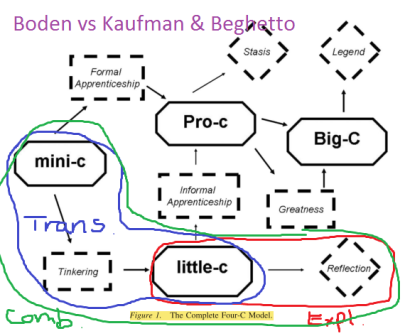
\includegraphics[width=.75\linewidth]{4CBoden.png}
% \caption[Kaufman vs Boden]{Kaufman's 4 C Model vs. Boden}
% \label{fig:4CB}
% \end{figure}

Quite recently, Anna Jordanous related the idea of the `4 P\rq s' to the discipline of computational creativity \autocite{Jordanous2015}.


\subsection{Creative Process}

The creative process has been subject to discussion and analysis as if it was `the holy grail' of creativity.

% \begin{enumerate}[label=(\alph*)]
\begin{description}
  \item [4 Stage Model] Henri Poincaré suggested a `4 Stage Model' (formulated by Graham Wallas in 1926). The stages are: preparation, incubation, illumination and verification \autocite{Poincare2001, Wallas1926}.
  \item [Problem Solving] George Pólya came up with a description of the `problem solving' process \autocite{Polya1957}.
\end{description}

\todo{add comb, trans, expl.? and koestler?}

Looking at table~\ref{tab:4SPPS}\marginnote{\faicon{table}~\ref{tab:4SPPS}} highlights the similarities of the two models above ((a) and (b)) and compares them to the `4 P Model'\marginnote{\faicon{object-group}~\ref{fig:4Crea}} of creativity from the previous section. Both the 4 Stage Model and the problem solving steps are linear. They're a sequence of steps followed one after the other. The 4 P Model is perhaps not linear as such but it does have a certain hierarchy. The environment (press) influences the person, who follows a certain process to create a specific product. In table~\ref{tab:4SPPS}\marginnote{\faicon{table}~\ref{tab:4SPPS}} the first two stages happen within the person and environment. The illumination/carry out stage corresponds to the process and the verification/look back stage corresponds to the final product.

\begin{table}[htbp]
\centering
\begin{tabu}{ccc}
\toprule
\textbf{4 Stage Model} & \textbf{Problem Solving} & \textbf{4 P Model} \\
\midrule
Preparation & Understand & Person \\
Incubation & Plan & Press \\
Illumination & Carry Out & Process \\
Verification & Look back & Product \\
\bottomrule
\end{tabu}
\caption[4 Step Model vs 4 P Model vs Problem Solving]{Comparison of 4 Step Model vs 4 P Model vs Problem Solving}
\label{tab:4SPPS}
\end{table}

\begin{draft}
  Giving ORDER to the 4 P model?!
\end{draft}



\subsection{Creative Disciplines}

\begin{draft}
  Initiatives that aim at a more rigorous understanding of computing and creativity have given rise to several fields, each having its own terminology and approach, but with significant overlaps.

  The two main disciplines directly related to creativity and technology that have emerged in recent years are as follows. `Creative Computing' tries to reconcile the objective precision of computer systems with the subjective ambiguity of human creativity \cite{Hugill2013c} and has an overarching theme of \textit{unite and conquer}, i.e. drawing from a wide range of transdisciplinary knowledge to tackle a problem (as opposed to the principle of \textit{divide and conquer} in computer science, which divides bigger problems down into smaller and easier parts) \cite{Yang2013}. The main challenge, Andrew Hugill and Hongji Yang argue, is for technology  to become `more adaptive, smarter and better engineered to cope with frequent changes of direction, inconsistencies, irrelevancies, messiness and all the other vagaries that characterise the creative process' \cite{Hugill2013c}. In part, these issues are due to the transdisciplinary nature of Creative Computing; factors such as common semantics, standards, requirements and expectations are typical challenges. Hugill and Yang therefore argue that creative software should be flexible and able to adapt to ever-changing requirements, evaluated and re-written continuously, and it should be cross-compatible.

  `Computational Creativity' has emerged from within Artificial Intelligence (AI) research. Simon Colton and Geraint Wiggins argue that AI falls within a problem-solving paradigm: `an intelligent task, that we desire to automate, is formulated as a particular type of problem to be solved', whereas `in Computational Creativity research, we prefer to work within an artefact generation paradigm, where the automation of an intelligent task is seen as an opportunity to produce something of cultural value' \cite{Colton2012}. They further explain that it models, simulates, replicates or enhances human creativity using a computer.
\end{draft}

Since creativity is studied in many different disciplines, projects such as this PhD research can be hard to categorise. As I have already discussed, this project is transdisciplinary\marginnote{§~\ref{ch:methodology}} and perhaps should be considered not part of one specific creative discipline but of many and beyond. Pure computer science, cognitive science or artificial intelligence clearly don't fit the bill. Recently however disciplines such as `creative computing', `computational creativity' and `digital humanities'\marginnote{§~\ref{ch:creativity}} have emerged.

% \begin{enumerate}[label=(\alph*)]
\begin{description}
  \item [Creative Computing] reconcile the objective precision of computer systems with the subjective ambiguity of human creativity. The process is made of 4 steps: motivation, ideation, implementation and operation \autocite{Hugill2013c}.
  \item [Computational Creativity] model, simulate, replicate or enhance human creativity using a computer \autocite{Colton2012}.
  \item [Digital Humanities] collaboration, transdisciplinarity and an engagement with computing and humanities \autocite{Burdick2012}.
\end{description}

These three disciplines share the theme of combining creativity with computing, but there are also differences. Creative computing for example is about doing computations in a creative way, while computational creativity is about achieving creativity through computation \autocite{Hugill2013}.

\begin{table}[htbp]
\centering
\begin{tabu}{ccc}
\toprule
\textbf{Artistic creation} & \textbf{Software engineering} & \textbf{Layer of abstraction} \\
\midrule
Motivation & User requirements & Abstract \\
Formulation & System design & Less abstract \\
Creation & Coding & Less concrete \\
Dissemination/revision & Operation/evolution & Concrete \\
\bottomrule
\end{tabu}
\caption[Artistic Creation vs Software Engineering vs Abstraction]{Comparison of Artistic Creation vs Software Engineering vs Abstraction by \autocite{Hugill2013c}}
\label{tab:acsea}
\end{table}

Table~\ref{tab:acsea}\marginnote{\faicon{table}~\ref{tab:acsea}} is taken directly from Hugill and Yang \autocite{Hugill2013c}. They use the comparison to software engineering and four layers of abstraction as the basis of their definition of the creative computing process, i.e. motivation, ideation, implementation and operation. I believe their observation that artistic creation and software engineering both represent a move from the abstract to the concerete is critical.

\begin{table}[htbp]
\centering
\begin{tabu}{XXXX}
\toprule
\textbf{Creative\newline Computing} & \textbf{Digital\newline Humanities} & \textbf{Computational\newline Creativity} & \textbf{Computer\newline Ethics} \\
\midrule
Motivation  & Design & Intentionality & Purpose \\
Ideation & Curation & Framing & People \\
Implementation & Computation & Process  & Process \\
Operation & Prototyping & Product  & Product \\
\bottomrule
\end{tabu}
\caption[Creative Computing vs Digital Humanities vs Computational Creativity vs Computer Ethics]{Comparison of Creative Computing vs Digital Humanities vs Computational Creativity vs Computer Ethics}
\label{tab:ccdhcc}
\end{table}

Table~\ref{tab:ccdhcc}\marginnote{\faicon{table}~\ref{tab:ccdhcc}} shows the four steps of creative computing defined by Andrew Hugill and Hongji Yang \autocite{Hugill2013c} and lines them up with corresponding activities in \gls{dh} \autocite{Burdick2012}, \gls{compc} \autocite{Colton2012} and Computer Ethics \autocite{Stahl2013}.

\begin{table}[htbp]
\small
\centering
\begin{tabu}{X[1.5]|XXXX}
\toprule
\textbf{Layer of\newline Abstraction} & \multicolumn{4}{c}{\textbf{ABSTRACT \hfill  $\longleftrightarrow$ \hfill CONCRETE}} \\
\midrule
4 Stage Model & Preparation & Incubation & Illumination & Verification \\
Problem Solving & Understand & Plan & Carry Out & Look Back \\
4 P Model & Person & Press & Process & Product \\
Artistic Creation & Motivation & Formulation & Creation & Dissemi\-nation \\
Software\newline Engineering & User Require\-ments & System Design & Coding & Operation \\
Creative\newline Computing & Motivation & Ideation & Implemen\-tation & Operation \\
Digital Humanities & Design & Curation & Computation & Prototyping \\
Computational\newline Creativity & Intentionality & Framing & Process & Product \\
Computer Ethics & Purpose & People & Process & Product \\
\bottomrule
\end{tabu}
\caption[Creative Process vs Creative Disciplines]{Comparison of Creative Process vs Creative Disciplines}
\label{tab:cpcd}
\end{table}

The spectrum from abstract to concrete as shown in table~\ref{tab:cpcd}\marginnote{\faicon{table}~\ref{tab:cpcd}} relates to the creative process models\marginnote{\faicon{table}~\ref{tab:4SPPS}} we have seen as well as the 4 P Model\marginnote{\faicon{object-group}~\ref{fig:4Crea}}.

\begin{description}
  \item [Abstract] Preparation, Understand, Person, Motivation, User Requirements, Design, Intentionality, Purpose
  \item [Less Abstract] Incubation, Plan, Environment, Formulation, System Design, Ideation, Curation, Framing, People
  \item [Less Concrete] Illumination, Carry Out, Process, Creation, Coding, Implementation, Computation
  \item [Concrete] Verification, Look Back, Product, Dissemination, Operation, Prototyping
\end{description}

\begin{draft}
  Abstract to Concrete is more about the practical process of artistic creation, not the conceptual development of a creative idea. That process is more of a move from concrete to abstract (known to unknown) using methods such as combinatorial, transformative and exploratory.
\end{draft}
\todo{add this to intro}


\section{Relating Pataphysics}

% \subsection{to Creativity}
\textbf{Text shown with a left bar is taken from \autocite{Hugill2013d}.}
\todo{rewrite}

\begin{draft}
  Combining computing with pataphysics seems impossible.

  \begin{itemize}
    \item Polymorphism (generalisations) oppose particularity.
    \item Precision (bugs) opposes exceptions and contradictions.
    \item Logic and structure oppose the imaginary and paradox.
    \item Cross-compatibility opposes the mutually exclusive.
    \item Responsiveness opposes the specific.
    \item Relevance opposes the creative.
  \end{itemize}
\end{draft}

Let's define creativity as `the ability to use original ideas to create something new and surprising of value'.

\begin{leftbar}
The creative process normally involves a move from the known to the unknown and sometimes from the named to the unnamed. In bringing something new into existence, the human qualities of openness and tolerance of ambiguity are generally regarded as highly desirable.
\end{leftbar}

\begin{leftbar}
Both the originality and the value of an idea are evaluated using subjective criteria. Pataphysics, which represents an extreme form of subjectivity, is therefore a highly appropriate framework within which to encourage and enable creative thinking and operations.
\end{leftbar}

\begin{quotation}
  The ambiguity of experience is the hallmark of creativity, that is captured in the essence of pataphysics. \sourceatright{\autocite{Hendler2013}}
\end{quotation}

\begin{quotation}
  Like all digitally encoded information, it has unavoidably the uncomfortable property that the smallest possible perturbations —i.e. changes of a single bit— can have the most drastic consequences. \sourceatright{\autocite{Dijkstra1988}}
\end{quotation}
\todo{check quote location}

% Pataphysics is highly subjective and particular and is as such very suitable for this kind of transformation from relevant to creative.

% \begin{quote}
%   [Pataphysics] can only be defined in a new undiscovered language because too obvious: tautology. \autocite{Baudrillard2007}
% \end{quote}

\begin{leftbar}
Boden argues that constraints support creativity, and are even essential for it to happen. `Constraints map out a territory of structural possibilities which can then be explored, and perhaps transformed to give another one' \autocite[p.82]{Boden2003}.
\end{leftbar}

\begin{leftbar}
This echoes the ideas of groups such as the Oulipo (which began as a Sub-Commission of the Collège de $'$Pataphysique), who investigate `potential literature' by creating constraints that frequently have a ludic element. Various other groups, the Ou-x-Pos, perform similar operations in fields as diverse as cinema, politics, music and cooking \autocite{Motte2007}.
\end{leftbar}

\begin{leftbar}
Boden's conceptual space is the `territory of structural possibilities'. So, the conceptual space of a teacup might be that it is meant to carry a certain amount of tea without breaking or burning fingers. It wouldn't be wise to create a teacup made out of paper. But whether we make a cup out of glass or porcelain, or how we shape the cup or the handle is pretty much up the individual's creativity. Being able to move around in this conceptual space, experiment (in thought or in reality) and play with different ideas while still following a given set of constraints is a good starting point for creativity to happen.
\end{leftbar}

% The Oulipo similarly classifies its conceptual space under two broad headings: the synthetic and the analytic:
%
% \begin{quote}
%   ``The analytic tendency investigates works from the past in order to find possibilities that often exceed those their authors had anticipated. […] The synthetic tendency is more ambitious: it constitutes the essential vocation of the Oulipo. It's a question of developing new possibilities unknown to our predecessors. This is the case, for example, of [Raymond Queneau's] 100,000,000,000,000 Poems or the Boolean haikus.'' \autocite[p.27]{Motte2007}
% \end{quote}
\todo{ref}
\begin{leftbar}
Later writings develop these ideas in more detail. La Littérature Potentielle \textbf{Oulipo1973}, is divided into several sections, dealing with clusters of methods, that include: anoulipisms (analytical oulipisms, such as combinatorial literature); use of preexisting structures such as lipograms (omitting a letter or letters), palindromes and snowballs (in which each successive word adds or subtracts a letter), homophonic translation, tautogram, and definitional literature; lexical, syntactic, or prosodic manipulations (such as the celebrated S+7, in which each substantive is replaced by the seventh word after it in a standard dictionary); lexicographical or prosodic synthoulipisms (early algorithmic methods); and perimathematical synthoulipisms (such as the Boolean poetry and combinatorial works already mentioned).
\end{leftbar}

\begin{leftbar}
Boden links her three aspects of creativity to three sorts of surprise. She says that creative ideas are surprising because they go against our expectations. `The more expectations are disappointed, the more difficult it is to see the link between old and new.' \autocite[p.84]{Boden2003} This suggests that fewer expectations (an open mind) allow creativity to happen more easily. Empirical experiences form expectations, which hinder our ability to accept creative ideas when they happen. In order to be able to recognise creative ideas we need to be able to see what they all have in common and in what way they differ and not reject unusual, unexpected ones.
\end{leftbar}

\begin{quotation}
  Unless someone realizes the structure which old and new spaces have in common, the new idea cannot be seen as the solution to the old problem. Without some appreciation of shared constraints, it cannot even be seen as the solution to a new problem intelligibly connected with the previous one. \sourceatright{\autocite[p.84]{Boden2003}}
\end{quotation}

\begin{leftbar}
It is clear that the Oulipo has a similar approach in its theorising of potential literature. Releasing creativity through constraint is its essential raison d'être.
\end{leftbar}

\begin{leftbar}
This is not to say that experience and knowledge are necessarily bad for creativity. To appreciate creativity we need to be knowledgeable in the relevant domain to be able to recognise old and new connections and transformations. But we also need a certain level of openness and tolerance for ambiguity to overcome our expectations.
\end{leftbar}

\begin{leftbar}
Perhaps it is for this reason that `creative people' are often assumed to have particular personality traits. Sternberg \autocite{Sternberg1999, Sternberg1999}, for example, proposes that these comprise: independence of judgement, self-confidence, and attraction to complexity, aesthetic orientation, and tolerance for ambiguity, openness to experience, psychoticism, risk taking, androgyny, perfectionism, persistence, resilience, and self-efficacy. More empirically, Heilman, Nadeau and Beversdorf \autocite{Heilman2003} have investigated the possible brain mechanisms involved in creative innovation. While a certain level of domain specific knowledge and special skills are necessary components of creativity, they point out that `co-activation and communication between regions of the brain that ordinarily are not strongly connected' might be equally important.
\end{leftbar}

\begin{leftbar}
Newell, Shaw and Simon add to the above with their report on the creative thinking process \autocite{Newell1963}. They identify three main conditions for creativity:
\end{leftbar}

\begin{itemize}
  \item the use of imagery in problem solving
  \item the relation of unconventionality to creativity
  \item the role of hindsight in the discovery of new heuristics
\end{itemize}

\begin{leftbar}
Other issues they point out are abstraction and generalisation. So, for example, poets transform the grammar of their conceptual space (in this case, language) to create new sentence structures in a poetic form. By doing so, they go against the expectations, the possibilities of the language and cause surprise. Some people might not understand the transformations and therefore the jokes or beauty of a poem simply because they are either not able to recognise connections between the old and newly transformed elements (maybe due to a lack of knowledge in the poems topic or in that particular language) or because they do not want to accept unconventional methods.
\end{leftbar}

\begin{table}[htb]
  \begin{tabu}{XX}
  \toprule
  \textbf{CREATIVITY} & \textbf{PATAPHYSICS} \\
  \midrule
  \textbf{Combinational}: Juxtaposition of dissimilar, bisociation, deconceptualisation
  &
  \textbf{Antinomy}: Symmetry, duality, mutually incompatible, contradicting, simultaneous existence of mutually exclusive opposites
  \par
  \textbf{Syzygy}: Alignment of three celestial bodies in a
  straight line, pun, conjunction of things, something unexpected
  and surprising
  \\ \midrule
  \textbf{Exploratory}: Noticing new things in old places
  &
  \textbf{Anomaly}: Exceptions, equality
  \\ \midrule
  \textbf{Transformative}: Making new thoughts possible by transforming old conceptual space, altering its own rules
  &
  \textbf{Clinamen}: Unpredictable swerve, the smallest possible aberration that can make the greatest possible difference
  \\
  \bottomrule
  \end{tabu}
\caption[Creativity vs Pataphysics]{Creativity vs Pataphysics}
\label{tab:creatpata}
\end{table}

\begin{leftbar}
Table~\ref{tab:creatpata}\marginnote{\faicon{table}~\ref{tab:creatpata}} compares some of the key ideas of creativity \autocite{Boden2003, Indurkhya, Koestler1964} with the main pataphysical operations. It will be seen that pataphysics succeeds in bringing into sharp relief the more generalised scientific ideas. The pataphysical terms are taken from the natural sciences or philosophy, but always with an ironic twist, betraying their underlying humour. They connect quite strongly with the primary descriptors of creativity, while adding a certain layer of jouissance. Pataphysics is self-avowedly useless, but its principles may prove surprisingly useful within this context.
\end{leftbar}


\section{Explaining Concepts}

\begin{description}
  \item [Patalgorithms] Pataphysical algorithms.
  \item [Pataphysicalisation] Applying pataphysical transformations to data.
  \item [Patadata] Data which has been pataphysicalised.
  \item [Patasaurus] A thesaurus for patadata.
  \item [Patametric Index] Patadata index.
  \item [Pranking] Pataphysical ranking.
\end{description}

\todo{rewrite sections here, integrate into other chapters}

\subsection*{Patalgorithms}

\begin{draft}
  The constraints for our conceptual space are the pataphysical rules that we want to apply to our data. We use those rules to explore, combine and transform our space; giving us the flexibility and freedom we need to find interesting results.

  We developed the idea of pataphysicalising data as the process of applying such pataphysical rules in order to produce creative search results. This pataphysicalisation\marginnote{\faicon{object-group}~\ref{fig:patasearch02}} process forms a central component of our system and influences all areas of the search tool.
\end{draft}

\todo{redraw figure}

% \begin{figure}[htb] % (here, top, bottom, page)
%   \centering
%   
\includegraphics[width=\linewidth]{patasearch01}
% \caption[Pata central1]{Pata central1}
% \label{fig:patasearch01}
% \end{figure}

\begin{figure}[htb] % (here, top, bottom, page)
  \centering
  % \def\svgwidth{\columnwidth}
  \input{images/patasearch01.pdf_tex}
\caption[Pata centrala2]{Pata centrala2}
\label{fig:patasearch02}
\end{figure}


\subsection*{Pataphylicalisation}

% The concept of pataphysicalisation, using pataphysical methods to transform an object/idea, on the search request however, does appear to be an interesting place to start the search for a new architecture. Whilst argued above, it cannot be the end of the process due to the amount it constrains the possible creative outputs, the characteristics of such a system, how you would get users to interactive with such a system, as well as how they would respond to it, will give valuable insight into the areas that need to be addressed by both the algorithms and hence the architecture.

The conceptual space for our project is `pataphysical Web searching'. There are some very simple rules or constraints that form an initial definition of the project. For example it is clear that we want to search the World Wide Web (rather than a library database), that we want to return a list of search results (and not a pile of books) and that we want the search process and its results to be creative/pataphysical (rather than relevant).  In a more technical sense, we have the query term (s), the index (of all web pages that we have crawled) and some pataphysical rules in our conceptual space. How we structure our search system, how we format the index or how we go about finding our results, is not in our conceptual space however. We can explore the space to its limits and we can transform it if we want to or feel like we need to. Our pataphysical rule set will include methods for transforming the space. By applying pataphysical rules to find results to our query we are pataphysicalising the query.

Definitions:
\begin{description}
  \item [To pataphysicalise] (verb) – applying pataphysical transformations
  \item [Pataphysicalisation] (noun) – the process of pataphysicalising
  \item [Patadata] (noun) – any data which has been pataphysicalised
\end{description}

But what exactly does the process of pataphysicalisation include? The kinds of transformations we are thinking of could be for example replacing or adding to the query term (s) with synonyms, antonyms, opposites, syzygies, clinamens etc. This can be done with the help of thesauri or dictionaries and ontologies. Whether we pataphysicalise our query term (s), the index or the results does not matter at this point. They are all possible and will maybe be done all at the same time\marginnote{\faicon{object-group}~\ref{fig:patasearch02f}}. We can consider the possibility of a `patametric index', rather than a parametric index or a `patasaurus' (pataphysical thesaurus/ontology).

\begin{figure}[htb] % (here, top, bottom, page)
  \centering
  \def\svgwidth{\columnwidth}
  \input{images/pataphysicalisation.pdf_tex}
\caption[Pataphysicalisation]{Pataphysicalisation}
\label{fig:patasearch02f}
\end{figure}

\begin{quotation}
  Arguably, few other textual forms will have greater impact on the way we read, receive, search, access, use and engage with the primary materials of humanities studies than the metadata structures that organize and present that knowledge in digital form. \sourceatright{\autocite[p.9]{Drucker2009}}
\end{quotation}


\subsection*{Patadata}

The idea of patadata is derived from the idea below:\\
Physics $\to$ Metaphysics $\to$ Pataphysics\\
Data $\to$ Metadata $\to$ Patadata

Patadata will allow us to engage with digital knowledge in a more creative way even. If metadata helps us organise information semantically then patadata is for organising information pataphysically. If metadata is objective then patadata is subjective. Drucker also points out that `many information structures have graphical analogies and can be understood as diagrams that organise the relations of elements within the whole.' \autocite[p.16]{Drucker2009} So maybe patadata could allow us to represent these graphical analogies in some way? An alphabetical list is a typical model for representing text data sets for example. Or an otherwise ranked list, a tree structure, a matrix, a one-to-many relationship, etc. But is a ranked list really the best way to represent search results? Ranking itself seems unpataphysical. It contradicts the philosophy of pataphysics, although we can argue that this contradiction makes it pataphysical again. Maybe this dilemma can be solved simply by adopting another type of graphical analogy to structure the results such as a tree structure instead of a ranked list.

Example: Let's say our patadata is represented by a list of keywords that each stands for a pataphysicalisation of the original query term. This list is added to each item in the index.

Query      = `Tree'\\
Patadata = [Tree (equivalent),  Car (opposite), Paper (antinomy),\\ Narwhal (anomaly), Book (syzygy), Venus Fly Trap (clinamen)]

Query      = `Sun God Ra'\\
Patadata = [Sun God Ra (equivalent), Slave (opposite), Holiday (antinomy),\\ Blue Balloon (anomaly), Pyramid (syzygy), Sphinx (clinamen)]


\subsection*{Pranking}

In traditional Web search, ranking signals contribute to the improvement of the ranking process. These can be content signals or structural signals. Content signals are referring to anything that is concerned with the text and content of a page. This could be simple word counts or the format of text such as headings and font weights. The structural signals are more concerned about the linked structure of pages. They look at incoming and outgoing links on pages. There are also Web usage signals that can contribute to ranking algorithms such as the clickstream. This also includes ideas such as the Facebook `like' button or the Google `+1' button which could be seen as direct user relevance feedback.

Ranking can be done at different stages of the search process. Depending on how the index is formatted and what information can be pre-computed at that stage, the ranking algorithm evaluates every Web page for relevance and returns them in order. There exist lots of different approaches on ranking, including PageRank \autocite{Brin1998} and HITS \autocite{Kleinberg1999}, which both analyse the link structure of the World Wide Web. They analyse the incoming and outgoing links on pages. PageRank for example assigns a numerical weight to each document, where each link counts as a vote of support in a sense. It is executed at indexing time, so the ranks are stored with each page directly in the index. HITS stands for `Hyperlink Induced Topic Search' and its basic features are the use of so called hubs and authority pages. It is executed at query time. Pages that have many incoming links are called authorities and pages with many outgoing links are called hubs.

Given a query term X, what is considered a relevant match though? Do we simply return a list of Web pages where X appears in the heading of each page? It is obviously not that easy. Several ranking signals are combined together; Google states that they use over 200 signals including PageRank and they personalise results using signals such as the web history and location (Google n.d.).
What kinds of ranking signals do we need for our pataphysical Web search tool? We could say that a page Y is relevant if it matches the patadata for query X. So, for example, Y would be a relevant result if it is a clinamen or syzygy to X. The more patadata matches there are the higher the ranking maybe. We don't necessarily have to assign a numerical ranking value to each page. Depending on how we structure our results page that might not be necessary. Shuffling the results list or the results tree could be an option.


\stopcontents[chapters]
